%!TEX root = ../thesis.tex
In this section we are going to cover our evaluation of our \emph{textile touch} explorative prototype, more specifically this is the latest prototype covered in \ref{ch:textiletouch:iteration3}~(\nameref{ch:textiletouch:iteration3}).
We have two primary goals of this evaluation.
On the one hand, we want to evaluate on the interaction potentials of using simple gestures as input control.
This goal involves using the prototype as an interactive device to control existing devices of the home.
On the other hand, we want to explore our prototype in alternative contexts.
This goal should shed light on the prototypes potential of encouraging alternative usages than controlling existing devices.

Evaluations were done over \todo{X} rounds to get a diversity in age groups of the test participants.
We were interested in shedding light on the diversity of creative ideas a child would bring compared to and adult.



\subsection{Future work}
\label{ch:textiletouch:futurework}

There are several points about the prototype that are candidates for future work.
We do see the prototyp

On the technical side there is room for improvement.
As the technology allows for multi-touch input it would be a great improvement for the user experience.
Multi-touch provides a much richer interaction style \todo{reference?} compared to single-touch and has become a standard in modern smart phone displays and laptop touchpads.
The gesture recognition framework used for the prototype, \$P, will work just fine with multi-touch and will not require further adjustment as the method of input is totally decoupled from the recognition framework. 
Figure~\ref{fig:ch:textiletouch:multitouch} shows a frame of input where several peaks made by finger inputs are detected. \todo{provide reason for not implementing multi-touch in the firstplace?}

\begin{figure}[h]
	\centering
  		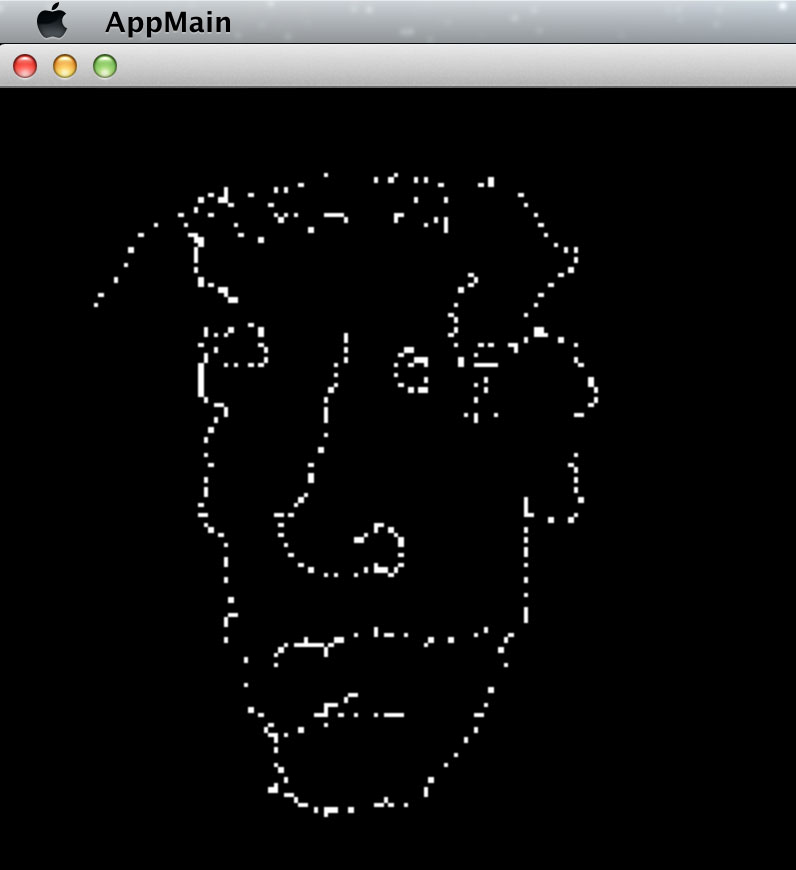
\includegraphics[width=3in]{figures/touch/face_drawing}
	\caption[Multi-touch: recognising multiple peaks of input.]
	{Multi-touch: recognising multiple peaks of input. \todo{insert correct screenshot!!!} }
   \label{fig:ch:textiletouch:multitouch}
\end{figure}

Mechanisms for providing direct feedback on the textile surface should be further investigated.
Vibrations \todo{\dots}

\todo{ting der er belyst fra evaluering \dots}

\begin{verbatim}
dette er ikke faerdig prototype - snakke om forskellige retninger
\end{verbatim}

